%--------------------------------------------------------------------------------------------------
% ips-phd-thesis-eng-apa.tex v1.3 (see the end of the file for modification
% history)
% To be used with ipsthesis.cls v1.3
% 
% A template for creating a PhD thesis in English using the APA 6th edition
% reference formatting
% with several accompanying files.  
% By Tea Tušar <tea.tusar@ijs.si>
%
% IMPORTANT NOTE: Biber must be used as the backhand for processing
% bibliographies, not bibtex!
%
% To compile this template, you need to run the following sequence of commands:
% 1. pdflatex  ips-phd-thesis-eng-apa
% 2. biber     ips-phd-thesis-eng-apa
% 3. makeindex ips-phd-thesis-eng-apa (optional, if you want an index)
% 4. pdflatex  ips-phd-thesis-eng-apa 
% 5. pdflatex  ips-phd-thesis-eng-apa
%-------------------------------------------------------------------------------

\documentclass[phd,eng,apa]{ipsthesis}
%
%-------------------------------------------------------------------------------
%  
% PREAMBULE
%-------------------------------------------------------------------------------
%
% Files with bibliographies 
\addbibresource{Moje-2017 - PhD citations.bib}
%\bibilography{Moje-2017 - PhD citations.bib}
%
% Define here all other packages and commands you need for your thesis, for 
% example:
\usepackage{color}
\usepackage{soul} %\hl command
\usepackage{longtable}
\usepackage{todonotes}
\usepackage{tikz} %\checkmark
\usepackage{listings} % for XML formatting
\usepackage{float} % for suppressing floating of tables/images
\usepackage{adjustbox} % For resizing tables
%For landscape related work table
\usepackage{pdflscape}
\usepackage{amsmath} % For nicer multi-line math
\DeclareLanguageMapping{american}{american-apa}
\DeclareLanguageMapping{slovene}{slovenian-apa}
%-------------------------------------------------------------------------------
%  
% DOCUMENT
%-------------------------------------------------------------------------------
\begin{document}
%-------------------------------------------------------------------------------
%
% FRONT MATTER
%-------------------------------------------------------------------------------
%
\frontmatter
%
\selectlanguage{american}
\pagestyle{fancy}

% Title pages
%--------------------------------------------------------------------------------------------------
% 
% INPUT FOR THE TITLE PAGES
%--------------------------------------------------------------------------------------------------
% 
% Author
\author{Luka Bradesko}         
%
% Title in English (use \protect\\ instead of \\ to create a line break)
\titleEnglish{Knowledge Acquisition through Natural Language Conversation and Crowdsourcing}
%
% Title in Slovene (use \protect\\ instead of \\ to create a line break)
\titleSlovene{Pridobivanje Strukturiranega Znanja skozi Pogovor ter s Pomocjo Mnozicenjai}
%
% Supervisor (title and name, affiliation)
\supervisorOne{Doc.\ Dunja Mladenic}{Jozef Stefan Institute, Ljubljana, Slovenia}
%
% Co-supervisor (title and name, affiliation), optional
%\supervisorTwo{Prof.\ Name Surname2}{Institution2, Place, Country}
%
% Co-supervisor (title and name, affiliation), optional
%\supervisorThree{Prof.\ Name Surname3}{Institution3, Place, Country}
%
% Evaluation board chairman (title and name, affiliation)
\evaluationBoardChairman{Dr.\ Michael Witbrock}{IBM, New York, New York}
%
% Evaluation board member #1 (title and name, affiliation)
\evaluationBoardMemberOne{Prof.\ Erjavec}{Jozef Stefan Institute, Ljubljana, Slovenia}
%
% Evaluation board member #2 (title and name, affiliation)
\evaluationBoardMemberTwo{Prof.\ Savnik}{Univerza v Novi Gorici, Nova Gorica, Slovenia}
% 
% Date
\thesismonth{April}
\thesisyear{2017}
%
\maketitle 

% Dedication (optional)
%--------------------------------------------------------------------------------------------------
% 
% INPUT FOR THE DEDICATION
%--------------------------------------------------------------------------------------------------
\dedication{To Vanessa}
\makededication


% Acknowledgments
%-------------------------------------------------------------------------------
% 
\chapter*{Acknowledgments}
\pdfbookmark[0]{Acknowledgments}{Acknowledgments}
%-------------------------------------------------------------------------------
I would like to express great appreciation to my PhD supervisor Prof. Dunja 
Mladenić for her support, guidance and advice throughout my studies. 
I would like to thank my co-autors, collaborators and
my colleagues from Jožef Stefan Institute for many valuable discussions, 
insights and suggestions. 
I would also like to thank the members of my doctoral committe, 
Michael Witbrock, Tomaž Erjavec and Iztok Savnik for their valuable comments and
remarks. 
Special thanks thanks go to Michael Witbrock, Janez Starc and Dane Sulič for
multiple years of help with the design and development of Curious Cat 
implementation. I thank to all of our 728 users who contributed 
to the experiment of the KA system, and Dr. Dave Schneider in particular and 
Cycorp management and members of the Cycorp technical staff (including Chris 
Deaton and Dr. David Baxter) more generally for licensing, for their kind 
assistance with APIs, KR advice and other assistance as we constructed and 
tested Curious Cat.
Additionally I would like to thank Marko Grobelnik and colleagues from
Artificial Intelligence Laboratory (Jožef Stefan Institute) for providing a 
good work and research environment, enabling me to focus on the research and
implementation required to finish this thesis. Similar thanks goes to AI team
at Bloomberg L.P., for encouraging me and allowing me to abstain from my work
duties while focusing on the thesis.

Finally I wish to thank Vanessa, my parents Agata and Bernard and my brothers
Marko and Valter for their support and encouragement.

\rule{0.5\textwidth}{.4pt}

This work was supported and partially financed by European Commission under
LARKC (The Large Knowledge Collider: a platform for large scale integrated
reasoning and Web-search, FP7-215535), MOBIS (Personalized Mobility Services 
for energy efficiency and security through advanced Artificial Intelligence 
techniques, FP7-318452), ENVISION (EmpoweriNg European SME business model 
Innovation ,ICT-2009-249120), OPTIMUM (Multi-source Big Data Fusion Driven 
Proactivity for Intelligent Mobility, H2020-MG-636160) and personally by 
Dr. Michael Witbrock.

 
% English abstract
%-------------------------------------------------------------------------------
% 
\chapter*{Abstract}
\pdfbookmark[0]{Abstract}{Abstract}
%-------------------------------------------------------------------------------

Knowledge Acquisition is an important part of Artificial Intelligence. Having high-quality structured knowledge helps to advance other research activities that depend on a rich understanding of the world around us. Due to a lack of reliable automation strategies this problem has been mostly attacked through hand-annotation and structuring by human experts. In recent years, there have been attempts to scale the manual approach through crowd-sourcing.

Although numerous systems and methods for crowd-sourced knowledge acquisition have been developed to solve the problem of manpower, the issues of high cost, task specification, targeting, consistency, and eventual quality of acquired knowledge, seem to persist.

The thesis addresses these issues by formalising and implementing an approach to scalable human-driven knowledge acquisition that significantly reduces the costs involved, and increases the quality of acquired knowledge. Through a novel set of tools, natural language user interaction, and a rich background knowledge base, our approach uses contextual clues to pick the right users at the right time: leveraging existing knowledge to check the consistency of user-provided answers. Newly acquired knowledge is incorporated into the knowledge base, creating a virtuous cycle whereby the knowledge acquisition process and the acquired knowledge are constantly improving through time. The proposed approach can be incorporated into natural language Human-Computer Interaction (HCI) interfaces to add high quality, cost-effective knowledge acquisition capabilities to almost any system with a distributed user base.

We propose a concrete implementation of the system, which has been tested over multiple years with thousands of users, yielding very promising results. During the test run, we collected over 57,978 answers, resulting in 386,980 new assertions. Evaluation shows the extracted knowledge to be true and useful 95\% of the time. Furthermore, using context to pro-actively drive knowledge acquisition increased engagement and effectiveness (the number of new assertions/day/user) by 175\% over the baseline.

% Slovene abstract, switch to slovene
\selectlanguage{slovene}
%-------------------------------------------------------------------------------
% 
\chapter*{Povzetek}
\pdfbookmark[0]{Povzetek}{Povzetek}
%-------------------------------------------------------------------------------

Povzetek v slovenščini naj ne bo daljši od ene strani. 
\hl{Translate from Englsh}

\selectlanguage{american}

% Contents
\maketoc
% List of figures (required if the thesis contains figures)
\makelof
% List of tables (required if the thesis contains tables)
\makelot
% List of algorithms (required if the thesis contains algorithms)
\makeloa
% Abbreviations (optional)
%--------------------------------------------------------------------------------
% 
\chapter{Abbreviations}
%-------------------------------------------------------------------------------
%
% A command that adjusts the of vertical positioning in the abbreviations and 
% symbols chapters
\chapteradjust
% Correct the width of columns (23pt and 377pt) to fit your needs 
% (they should sum up to 400pt).
% Use \cr instead of \\ to break lines.
\begin{longtable}{@{}p{40pt}@{\hspace{13pt} \dots \hspace{5pt}}p{360pt}@{}}

AI & Artificial Intelligence \cr
CC & Curious Cat (a name of the knowledge acquisition application and platform 
that is a side result of this thesis) \cr
CSK & Common Sense Knowledge \cr
CYC & An AI system (Inference Engine and Ontology), developed by Cycorp Inc. \cr
CycKB & Cyc Knowledge Base (Ontology part of Cyc system) \cr
CycL & Cyc Lanugage \cr
FCM & Firebase Cloud Messaging\cr
GUI & Graphical User Interface \cr
GWAP & Games With A Purpose \cr
HCI & Human-Computer Interaction \cr
HMI & Human to Machine Interaction \cr
JSI	& Jožef Stefan Institute \cr
KA & Knowledge Acquisition \cr
KB & Knowledge Base \cr
KE & Knowledge Entry \cr
KR & Knowledge Representation \cr
KU & Kyoto University\cr
LSA & Latent Semantic Analysis \cr
MHI & Machine to Human Interaction \cr
MIT & Massachusetts Institute of Technology \cr
MMHHI & Machine Mediated Human to Human Interaction \cr
Mt & Microtheory \cr
Mts & Microtheories \cr
MPI & Max Planck Institute \cr
MSR & Microsoft Research \cr
NL & Natural Language\cr
NLP & Natural Language Processing \cr
NP & Noun Phrase\cr 
NTU & National Taiwan University \cr
NUS & National University of Singapore \cr
OIE & Open Information Extraction\cr
PMI & Point-wise Mutual Information\cr
POI & Point of Interest\cr
POS & Part of Speech \cr
POS:X & Abbreviations for Part of Speech tags used by POS parsers \cr
POS:CC & Coordinating conjunction \cr
POS:CD & Cardinal Number \cr
POS:DT & Determiner \cr
POS:EX & Existential there \cr
POS:FW & Foreign Word \cr
POS:IN & Preposition or subordinating conjunction \cr
POS:JJ & Adjective \cr
POS:JJR & Adjective, comparative \cr
POS:JJS & Adjective, superlative \cr
POS:LS & List item marker \cr
POS:MD & Modal \cr
POS:NN & Noun, singular or mass\cr
POS:NNS & Noun, plural \cr
POS:NNP & Proper noun, singular \cr
POS:NNPS & Proper noun, plural \cr
POS:PDT & Predeterminer \cr
POS:POS & Possessive ending \cr
POS:PRP & Personal pronoun \cr
POS:PRP\$ & Possessive pronoun \cr
POS:RB & Adverb \cr
POS:RBR & Adverb, comparative \cr
POS:RBS & Adverb, superlative \cr
POS:RP & Particle \cr
POS:SYM & Symbol \cr
POS:TO & to \cr
POS:UH & Interjection \cr
POS:VB & Verb, base form \cr
POS:VBD & Verb, past tense \cr
POS:VBG & Verb, gerund or present participle \cr
POS:VBN & Verb, past participle \cr
POS:VBP & Verb, non-3rd person singular present \cr
POS:VBZ & Verb, 3rd person singular present \cr
POS:WDT & Wh-determiner \cr
POS:WP & Wh-pronoun \cr
POS:WP\$ & Possessive wh-pronoun \cr
POS:WRB & Wh-adverb \cr
PTT & Taiwanese Bulletin Board System \cr
SKSI & Semantic Knowledge Source Integration \cr
SPD & Staypoint Detection \cr
TUW & The University of Waikato, New Zealand \cr
UL & University of Leipzig \cr
UoM & University of Mannheim \cr
UoR & University of Rochester \cr
UW & University of Washington \cr
\end{longtable}

% Symbols (optional)
%-------------------------------------------------------------------------------
% 
\chapter{Symbols}
\label{chapter:symbols}
%-------------------------------------------------------------------------------
%
% A command that adjusts the vertical positioning in the abbreviations and 
% symbols chapters
\chapteradjust
% Correct the width of columns (10pt and 390pt) to fit your needs (they 
% should sum up to 400pt).
% Use \cr instead of \\ to break lines.
\begin{longtable}{@{}p{17pt}@{\hspace{2pt} \dots \hspace{5pt}}p{383pt}@{}}

$\in$ & Element of. Stating $x \in S$ means that $x$ is an element of the 
set $S$. \cr

$\land$ & logical conjunction (and). The statement $A \land B$ is true if both
$A$ and $B$ are true, otherwise it is false.  \cr

$\forall$ & Universal Quantifier (for all). One of the quantifiers used to be
able to convert atomic formulas into propositions. For example, 
$\forall x \in S:P(x)$  means that the propositional function $P(x)$ is true
for every $x$ in the set $S$. Or shorter. $\forall x:P(x)$, means this is true
in the universal set. Given yet another example, non propositional atomic
formula $x > 5$ which is neither true or false, can be converted into true/false
proposition by adding a quantifier: $\forall x:x>5$.\cr

$\exists$ & Existential Quantifier (there exists). One of the quantifiers, 
that can be used to convert atomic formulas into propositions. For example,
$\exists x \in S:P(x)$ means that there exists at least one $x$ in the set $S$,
for which the propositional function $P(x)$ is true. Or shorter, 
$\exists x:P(x)$ means that there exists at least one $x$ in the universal set,
for which the porpositionalfunction is true. Given yet another, non 
propositional atomic formula $x > 5$ is neither true or false. But when 
converted to proposition by adding a quantifier it becomes either true or false 
in the given set: $\exists x:x>4$.\cr

$\implies$ & \emph{Material implication}, also known as 
\emph{Material conditional} or simlply \emph{implication} is a logical 
connective that is used to form the statements like $p \implies f$, which can
be read as "if $p$ is true, then also $q$ is true". If $p$ is true and $q$ is
false, then the whole statement $p \implies q$ is false. \cr
\end{longtable}

% Glossary (optional)
%-------------------------------------------------------------------------------
% 
\chapter{Glossary}
%-------------------------------------------------------------------------------
\emph{Antecedent (predicate logic)} is a first half of the hypotetical 
proposition. It is a $p$ part of the implies statement (see symbol $\implies$ in
Chapter Symbols for explanation. In an implication $p \implies q$, $p$ is an
antecedent.\\

\emph{Arity (predicate logic)} is a property of predicate that defines the 
number of parameters or operands that predicate can operate with. For example,
if a predicate $P$ has \emph{arity} of 2, valid statements using this predicate
can only be the ones with exactly 2 operands ($P(x,y), P(a,b),...$). Statement
$P(x)$ is in this case not a valid statement, since it uses the predicate with
only one parameter.\\

\emph{AST (Abstract Syntax Tree)} is an abstract representation of Wikipedia 
page as parsed from DBPedia parser. Something like DOM tree for Wikipedia 
instead for pure HTML\\

\emph{Atomic Formula} (predicate logic). If the predicate $P$ has arity $n$,
then $P$ followed by $n$ constants and variables is an atomic formula. Examples:
$P(a), P(x), P(x,y) D(a,x)$.\\

\emph{Consequent (predicate logic)} is a second half of the hypotetical 
proposition. It is a $q$ part of the implies statement (see symbol $\implies$ in
Chapter Symbols for explanation. In an implication $p \implies q$, $q$ is a
consequent or apodosis.\\

\emph{Constant} (predicate logic) is besides \emph{variables}, 
\emph{predicates}, and \emph{quantifiers} one of the atomic parts of the 
\emph{predicate logic} sentences. For example, in a sentence $P(a,x)$, $a$ 
serves as a constant. Constants are usually marked with the letters from the
beginning of the alphabet. In this thesis, also predicate is a constant and
all constants are written either with letters or their $Names$.\\

\emph{Existential Quantifier ($\exists$)}. For explanation see the symbol
$\exists$ in the chapter Symbols.\\

\emph {First order logic} can also be called \emph{Predicate logic}. See this
term for more refined definition\\

\emph{Material implication ($\implies$)}. For explanation, see $\implies$ in the
Chapter Symbols.\\

\emph{OIE (Open Information Extraction} is a paradigm introduced by Oren Etizoni
in his TextRunner system. The main idea of this paradigm is that the knowledge 
acquisition system is not pre-determined to extract some specific facts, 
patterns, etc, but is open-ended, extracting large set of relational tuples 
without any human input.\\

\emph{PMI (Pointwise Mutual Information} is a measure which captures 
co-occurence relationsip between terms in a big corpus.\\

\emph{predicate} is a a term used in predicate logic, representing a verb
template that desribes properties of objects, or relationships between multiple
objects.\\

\emph{Predicate logic}, called also \emph{First order logic} is a formal system
that uses quantification over variables. This makes this logic more expressive
than the \emph{Propositional logic}. In some limited sense, 
\emph{Predicate logic} could be defined as \emph{Propositional logic} with 
quantifiers.\\

\emph{proposition}. This term is often synonim for a logical \emph{statement},
but can also mean more abstract meaning that two different statements with the
same meaning represent. In \emph{Propositional logic}, a proposition is the
smalles syntactic unit. On the other hand, in \emph{Predicate logic}, 
statements/sentences are broken into \emph{constatants, variables, predicates}
and \emph{quantifiers}.\\

\emph{Propositional function}, is an atomic function in from the 
\emph{Predicate logic} which is open ended (missing quantifiers) and thus
cannot count as proposition. For example, $P(x)$ is a propositional function,
while $\forall x P(x)$ is a proposition.\\

\emph{Propositional logic}, also known as \emph{sentential} or 
\emph{statement logic}, is the branch of logic that operates with entire
propositions/statements/sentences to form more complicated 
propositions/statements/sentences, and also logical relationships and properties
derived from combining  or altering this statements.\\

\emph{Quantifier} (logical). Quantifiers in \emph{Predicate logic} convert
propositional functions (open ended) into proper propositions which can be true
or false. For example, $P(x)$ is a propositional function, which can get
converted into proper proposition using one of the quantifiers: 
$\forall x P(x)$. For more info look for the terms \emph{Universal Quantifiier}
and \emph{Extistential Quantifier}.\\

\emph{Sentential logic}. See the term \emph{Propositional logic}.\\

\emph{SKSI (Semantic Knowledge Source Integration)} is a \emph{Cyc} sub-system
for external knowledge integration.\\

\emph{Statement logic}. Synonim for \emph{Propositional logic}. For description
see the glossary for this term.\\

\emph{Upper Ontology} (also top-level, foundation or core ontology) is the part
of ontology (or knowledge base), which defines the core objects that serve as a
main knowledge building blocks to construct the full knowledge base.\\

\emph{Universal Quantifier ($\forall$)}. For explanation check the symbol 
$\forall$ in the chapter Symbols. \\


%-------------------------------------------------------------------------------
% MAIN MATTER
%-------------------------------------------------------------------------------
\mainmatter

% Introduction
%-------------------------------------------------------------------------------
% 
\chapter{Introduction}
%-------------------------------------------------------------------------------
An intelligent being or machine solving any kind of a problem needs knowledge to which it can apply its intelligence while coming up with an appropriate solution. This is especially true for the knowledge-driven AI systems which constitute a significant fraction of general AI research. For these applications, getting and formalizing the right amount of knowledge is crucial. This knowledge is acquired by some sort of Knowledge Acquisition (KA) process, which can be manual, automatic or semi-automatic. Knowledge acquisition, using an appropriate representation and subsequent knowledge maintenance are two of the fundamental and as-yet unsolved challenges of AI. Knowledge is still expensive to retrieve and to maintain. This is becoming increasingly obvious, with the rise of chat-bots and other conversational agents and AI assistants. The most developed of these (Siri, Cortana, Google Now, Alexa), are backed by huge financial support from their producing companies, and the lesser-known ones still result from 7 or more person-years of effort by individuals
\todo:{\hl{Finish}}

Knowledge acquisition and subsequent knowledge maintenance, are two of the fundamental and as-yet not-completely-solved challenges of Artificial Intelligence (AI).

\hl{We propose and implement novel approach to automated knowledge acquisition using the user context obtained from a mobile device and knowledge based conversational crowdsourcing. The resulting system named Curious Cat has a multi objective goal, where KA is the primary goal, while having an intelligent assistant and a conversational agent as secondary goals. The aim is to perform KA effortlessly and accurately while having a conversation about concepts which have some connection to the user, allowing the system (or the user) to follow the links in the conversation to other connected topics. We also allow to lead the conversation off topic and to other domains for a while and possibly gather additional, unexpected knowledge. For illustration see the example conversation sketch in Table I, where topic changes from a specific restaurant to a type of dish. In this example case, the conversation is started by the system when user stays at the same location for 5 minutes.}

\section{Scientific Contributions}
This section gives an overview of scientific and other contributions of this thesis to the knowledge acquisition approaches.

\subsection{Novel Approach Towards Knowledge Acquisition}
Traditionally KA (knowledge acquisition) approach focuses on one type of acquisition process, which can be either Labor, Interaction, Mining or Reasoning\parencite{Zang2013}. In this thesis we propose a novel, previously untried approach that intervenes all aforementioned types with current user context and crowdsourcing into a coherent, collaborative and autonomous KA system. It uses existing knowledge and user context, to automatically deduce and detect  missing or unconfirmed knowledge(reasoning) and uses this info to generate crowdsourcing tasks for the right audience at the right time(labor). These tasks are presented to users in natural language (NL) as part of the contextual conversation (interaction) and the answers parsed (mining) and placed into the KB after consistency checks(reasoning). The approach contribution can be summed up as a) definition of the framework for autonomous and collaborative knowledge acquisition with the help of contextual knowledge (\hl{chapter X}), and b) demonstrate and evaluate the contributions of contextual knowledge and approach in general \hl{chapter X}.

\subsection{Knowledge Acquisition Platform Implementation as Technical Contribution }
Implementation of the KA framework as a working real-world prototype which shows the feasibility of the approach and a way to connect many independent and complex sub-systems. Sensor data, natural language, inference engine, huge pre-existing knowledge base (Cyc)\hl{CycRef}, textual patterns and crowdsourcing mechanisms are connected and interlinked into a coherent interactive application (\hl{Chapter X}).

\subsection{A Shift From NL Patterns to Logical Knowledge Representation in Conversational Agents}
Besides the main contributions presented above, one aspect of the approach introduces a shift in the way how conversational agents are being developed. Normally the approach is to use textual patterns and corresponding textual responses, sometimes based on some variables, and thus encode the rules fro conversation. As a consequence of natural language interaction, the proposed KA framework is in some sense a conversational agent which is driven by the knowledge and inference rules and uses patterns only for conversion from NL to logic. This shows promise as an alternative approach to building non scripted conversational engines (\hl{Chapter X}).

\section{Thesis structure}
The rest of the thesis is structured in to chapters covering specific topics. \hl{Chapter X} introduces\todo{...Finish}

% If needed, the thesis can consist of parts (not encouraged)
%\part{First Part of the Thesis}

% Second chapter 
%-------------------------------------------------------------------------------
\chapter{Background and Related Work}

In this chapter we will give an overview of approaches and related works on
broader knowledge acquisition research field, information extraction, 
crowdsourcing and geo-spatial context mining. 

Knowledge Acquisition has been addressed from different perspectives by many 
researchers in Artificial Intelligence over decades, starting already in 1970 
as a sub-discipline of AI research, and since then resulting in a big number of 
types and implementations of approaches and technologies/algorithms. The 
difficulty of acquiring and maintaining the knowledge was soon noticed and was 
coined as \emph{Knowledge Acquisition Bottleneck} in 
1977\parencite{Feigenbaum1977}. In more recent survey of KA approaches 
\parencite{Zang2013}, authors categorize all of the KA approaches into four main
groups, regarding the source of the data and the way knowledge is acquired:
\begin{itemize}
	\item \emph{Labour Acquisition.} This approach uses human minds as the 
    knowledge source. This usually involves human (expert) ontologists manually 
    entering and encoding the knowledge.
	\item \emph{Interaction Acquisition.} As in Labour Acquisition, the source 
    of the knowledge is coming from humans, but in this case the KA is wrapped 
    in a facilitated interaction with the system, and is sometimes implicit 
    rather than explicit.
	\item \emph{Reasoning Acquisition.} In this approach, new knowledge is 
    automatically inferred from the existing knowledge using logical rules and 
    machine inference.
	\item \emph{Mining Acquisition.} In this approach, the knowledge is 
    extracted from some large textual corpus or corpora.
\end{itemize}

We believe this categorization most accurately reflects the current state of 
machine (computer) based knowledge acquisition, and we decided to use the same 
classification when structuring our related work, focusing more on closely 
related approaches and extending where necessary. According to this 
classification, our work presented in this thesis, fits into a hybrid approach 
combining all four groups, with main focus on interaction and reasoning. We 
address the problem by combining the labour and interaction acquisition (users 
answering questions as part of NL interaction aimed at some higher level goal, 
such as helping the user with various tasks), adding unique features of using 
user context and existing knowledge in combination with reasoning to produce a 
practically unlimited number of potential interaction acquisition tasks, going 
into the field of crowd-sourcing by sending these generated tasks to many users 
simultaneously.

\todo{Fix this, reference to chapters instead to specifici works.} 
Previous works that can compare with our solution is divided into the systems 
that exploit existing knowledge (generated anew during acquisition or 
pre-existing from before in other sources) \parencite{Singh2002a,Witbrock2003,
Forbus2007,Kvo2010,Sharma2010,Mitchel2015}, reasoning \parencite{Witbrock2003,
Speer2007,Speer2008,Kuo2010}, crowdsourcing \parencite{Singh2002,Speer2009, 
Kuo2010, Pedro2012a, Pedro2013}, acquisition through interaction 
\parencite{Speer2009,Pedro2012,Pedro2013}, acquisition through labour(\hl{add, 
probably rather refer to subsections}) \parencite{} and natural language 
conversation\parencite{Pedro2012, Speer2007,Speer2009, Witbrock2003,Kuo2010}.

\hl{Test referencing table} (see \tablename~\ref{tab:related}).

\begin{landscape}
	\begin{table}[htb]
	\caption{Structured overview of related KA systems}
	\label{tab:related}
	\centering
	\begin{tabular}{lclcccccc}
		\hline
		System & Parent & Reference & Category & Source & Representation & Prior K. &  Crowds. & Context \\
		\hline
		Cyc project (Cycorp) & / & \parencite{Lenat1995} & Labour & K. Exp. & CycL & / & / & / \\
		ThoughtTrasure(Signiform) & / & \parencite{Mueller2003} & Labour & K. Exp. & LAGS & / & / & / \\
		HowNet (Keen.) & / & \parencite{Dong2010} & Labour & K. Exp. & KDML & / & / & / \\
		OMCS (MIT) & / & \parencite{Singh2002a} & Labour & Public & ConceptNet & / & \checkmark & / \\
		KRAKEN (Cycorp) & Cyc & \parencite{Panton2002a} & Interaction & D. Exp & CycL & \checkmark & / & / \\
		UIA (Cycorp) & Cyc & \parencite{Witbrock2003UIA} & Interaction & D. Exp & CycL & \checkmark & / & / \\
		Factivore (Cycorp) & Cyc & \parencite{Witbrock2005} & Interaction & D. Exp & CycL & \checkmark & / & / \\
		Predicate Populator (Cycorp) & Cyc & \parencite{Witbrock2005} & Interaction & D. Exp & CycL & \checkmark & / & / \\
		CURE (Cycorp) & Cyc & \parencite{Witbrock2010} & Interaction & D. Exp & CycL & \checkmark & / & / \\
		OMCommons (MIT) & OMCS & \parencite{Speer2007} & Interaction & Public & ConceptNet & \checkmark & \checkmark & / \\
		Freebase (Metaweb/Google) & / & \parencite{Bollacker2008} & Interaction & Public & RDF & / & / & / \\
		20 Questions (MIT) & OMCS & \parencite{Speer2009} & Game & Public & ConceptNet & / & / & / \\
		\hline
	\end{tabular}
\end{table}
\end{landscape}

\section{Labour Acquisition}
\label{section:LabourAcquisition}
This category consists of KA approaches which rely on explicit human work to 
collect the knowledge. A number of expert (or also untrained) ontologists or 
knowledge engineers is employed to codify the knowledge by hand into the given 
knowledge representation (formal language). Labour acquisition is the most 
expensive acquisition type, but it gives a high quality knowledge. It is often a
crucial initial step in other KA types as well, since it can help to have some 
pre-existing knowledge to be able to check the consistency of the newly acquired
knowledge. Labour Acquisition is often present in other KA types, even if not 
explicitly mentioned, since it is implicitly done when defining internal 
workings and structures of other KA processes. While we checked other well 
known systems that are result of Labour Acquisition, Cyc (mentioned below) is 
the most comprehensive of them and was picked as a starting point and main 
background knowledge and implementation base for this work.

\emph{Cyc.} The most famous and also most comprehensive and expensive knowledge 
acquired this way, is Cyc KB, which is part of Cyc AI system 
\parencite{Lenat1995}. It started in 1984 as a research project, with a premise 
that in order to be able to think like humans do, the computer needs to have 
knowledge about the world and the language like humans do, and there is no other
way than to teach them, one concept at a time, by hand. Since 1994, the project 
continued through Cycorp Inc. company, which is still continuing the effort. 
Through the years Cyc Inc. employed computer scientists, knowledge engineers, 
philosophers, ontologists, linguists and domain experts, to codify the knowledge
in the formal higher order logic language CycL \parencite{Matuszek2006a}. As of 2006
\parencite{Matuszek2006}, the effort of making Cyc was 900 non-crowdsourced 
human years which resulted in 7 million assertions connecting 500,000 terms and 
17,000 predicates/relations \parencite{Zang2013}, structured into consistent 
sub-theories (Microtheories) and connected to the Cyc Inference engine and 
Natural Language generation. Since the implemtentation of our approach is based
on Cyc, we give a more detailed description of the KB and its connected systems
in \autoref{section:Cyc} on page \pageref{section:Cyc}. Cyc Project is still 
work in progress and continues to live and expand through various research and
commercial projects.

\emph{ThoughtTreasure.} Approximately at the same time(1994) as Cyc Inc. company
was formed, Eric Mueller started to work on a similar system, which was inspired
by Cyc and is similar in having a combination of common sense knowledge concepts
connected to their natural language presentations. The main differentiator from 
Cyc is, that it tries to use simpler representation compared to first-order 
logic as is used in Cyc. Additionally, some parts of ThoughtTreasure knowledge 
can be presented also with finite automata, grids and scripts 
\parencite{Mueller1999,Mueller2003}. In 2003 the knowledge of this system 
consisted of 25,000 concepts and 50,000 assertions. ThoughtTreasure was not so 
successfull as Cyc and ceased all developments in 2000 and was open-sourced on 
Github in 2015. \hl{link as footnote}.

\emph{HowNet} started in 1999 and is an on-line common-sense knowledge base 
unveiling inter-conceptual relationships and inter-attribute relationships of 
concepts as connoting in lexicons of the Chinese and their English equivalents. 
As of 2010 it had 115,278 concepts annotated with Chinese representation, 
121,262 concepts with English representation, and 662,877 knowledge base records
including other concepts and attributes \parencite{Dong2010}. HowNet knowledge 
is stored in the form of concept relationships and attribute relationships and 
is formally structured in KDML (Knowledge Database Mark-up Language), consisting
of concepts (called semens in KDML) and their semantic roles.
 
\emph{Open Mind Common Sense (OMCS)} is a crowdsourcing knowledge acquisition 
project that started in 1999 at the MIT Media Lab\parencite{Singh2002a}. 
Together with initial seed and example knowledge, the system was put online with
a knowledge entry interface, so the entry was crowd-sourced and anyone 
interested could enter and codify the knowledge. OMCS supported collecting 
knowledge in multiple languages. It's main difference from the systems described
above (Cyc, HowNet, ThoughtTreasure) is, that it used deliberate crowdsourcing
and that it's knowledge base and representation is not strictly formal logic, 
but rather inter-connected pieces of natural language statements. As of 2013 
\parencite{Zang2013}, OMCS produced second biggest KB after Cyc, consisting of 
English (1,040,067 statements), Chinese (356,277), Portuguese (233,514), 
Korean (14,955), Japanese (14,546), Dutch (5,066), etc. Initial collection was
done by specifying 25 human activities, where each activity got it's own user 
interface for free form natural language entry and also pre-defined patterns 
like "A hammer is for \underline{\hspace{1.5cm}}", where participants can enter
the knowledge. Although OMCS started to build KB from scratch it shares a 
similarity to our CC system in a sense that it is using crowd-sourcing and also
natural language patterns with empty slots to fill in missing parts. OMCS was
later used in many other KA approaches as a prior knowledge, similar way as we 
use Cyc. After a few versions, OMCS was taken from public access and merged with
multiple KBs and KA approaches into an ConceptNet 
KB\footnote{http://conceptnet.io/} \parencite{Speer2016}, which is now (in 2017)
part of Linked Open Data (LOD) and maintained as open-source project.
 
\section{Interaction Acquisition}
Similarly as with Labour KA, interaction Acquisition gets the knowledge from 
human minds, but in this case the acquisition is an intended side effect, while
users are interacting with the software as part of some other activity/task, or
as part of a motivation scheme, such as knowledge acquisition games. Besides 
games, the interaction could be some other user interface for solving specific
tasks, or a Natural Language Conversation. This type of acquisition is most 
strongly correlated with the approach described in this thesis, since Curious 
Cat uses points (gaming), to motivate users and it interacts with user in NL, 
while discussing various topics (concepts). It uses the conversation to set up
the context and acquire (remember) user's responses and places them properly in
to the KB. Sometimes the acquired knowledge is paraphrased and presented back to
user to show the 'understanding', which was first tried in OSMC (
\autoref{section:LabourAcquisition}, \parencite{Singh2002b}), but there only in
non-conversational way as part of the input forms.
 
\subsection{Interactive User Interfaces}
Interactive user interfaces are the most common representation of interaction 
acquisition, where the user interface is constructed in a way to help user enter
the data and thus make the acquisition much faster and cheaper. Historically, 
these systems were developed to help the labour acquisition systems, or on top
of them, after parent systems reached some sort of maturity and initial 
knowledge stability. This is the reason why all of these systems rely or are 
build on top of labour acquisition (\autoref{section:LabourAcquisition}) or 
mining acquisition (\autoref{section:MiningAcquisition}) systems.

\emph{KRAKEN} system was a knowledge entry tool which allows domain experts to
make meaningful additions to CYC knowledge base, without the training in the 
areas of artificial intelligence, ontology development, or knowledge
representation\parencite{Panton2002a}. It was developed as part of DARPA's
Rapid Knowledge Formation (RKF) project in 2000. As its goal was to allow
knowledge entry to non-trained experts, it started to use natural language 
entry and is as this, a first pre-cursor to Curious Cat system and a seed idea
for it. It consists of creators, selectors, modifiers of Cyc KB building blocks,
tools for consistency checks and tools for using existing knowledge to infer new
things to ask. This tool, together with it's derived solutions was later 
re-written and integrated into Cyc as CURE system (see below). While KRAKEN and
later CURE already used Natural Language generation and parsing, and started 
with the idea of natural language dialogue for doing the KA, the interaction, it
was missing user context (user's had to select or search the concept of 
interest), and also crowdsourcing aspects. Kraken was also missing rules for
explicit question asking. The questions were all related to the selected concept
and given as a list of natural language forms.

\emph{User Interaction Agenda (UIA)} was a web  based user interface for KRAKEN
KA tool\parencite{Panton2002a,Witbrock2003UIA}. It worked inside a browser and 
it worked as responsive web-app (in 2001) by automatically triggering refresh 
functionality of the browser. It consisted of a menu of tools that is organized
according to the recommended steps of the KE process, text entry box (query, 
answer, statement), center screen for the main interaction with the current 
tool, and a summary with a set of colored steps needed to complete current 
interaction. Similarly as KRAKEN itself, this interface was later improved
and integrated into main Cyc system as part of CURE tool. 

\emph{Factivore} was a Java Applet user interface for an extended KRAKEN system,
meant for quick facts entering \parencite{Witbrock2005}. On the back-end it used
the same mechanisms and logical templates, while in the front-end it only
allowed facts entering, as opposed to UIA, which also allowed rules (which
ended up as not being useful).

\emph{Predicate Populator} is a similar tool as \emph{Factivore}, which instead
of only collecting instances, allows to add general knowledge about classes. For
example, instead of describing facts for a specific restaurant, it can collect
general knowledge that is true for all restaurants \parencite{Witbrock2005}. The
context of the KA in this case, is given by class concept, a predicate and a 
web-site which is parsed into CycL concepts. These are then filtered out if they
do not match argument constraints of the predicate and then shown to user for 
selection. As part of the validation, this tool had some problems with correctly
acquired knowledge. One of the proposed solutions (never implemented), was to
start using volunteers to vote about the correctness. This is already a 
pre-cursor idea for crowd-sourced voting mechanisms that we used in Curious Cat.

\emph{Freebase} started in 2007\parencite{Bollacker2008} and was a large (mostly
instance based) crowd-sourced graph database for structured general human 
knowledge. Initially it was acquired from multiple public sources, mostly 
Wikipedia. The initial seed was then constantly updated and corrected by the 
community. On the user interface side, Freebase provides an AJAX/Web based 
UI for humans and an HTTP/JSON based API for software access. For finding
knowledge and also software based editing, it uses Metaweb Query Language 
(MQL). A company behind freebase was bought by Google in 2010 and incorporated
into a Google Knowledge Graph. In 2016 Freebase was incorporated into the 
Wikidata platform and shut down by Google and is no longer maintained.

\emph{OMCommons (Open Mind Commons)} is an interactive interface to OMCS which
can respond with a feedback to user answers and maintain dialogue 
\parencite{Speer2007}. This is similar approach as we do with Curious Cat and
shows understanding of the knowledge users enter. The mechanisms behind is
by using inference engine to make analogical inferences based on the existing 
knowledge and new entry. Then it generates some relevant questions and asks 
user to confirm them. For example, as given from the original paper, 
\emph{OMCommons} asks: "A bicycle would be found on the street. Is this common 
sense?". This is then displayed to the user with the justification for the 
question: "A bicycle is similar to a car. I have been told that a car would 
be found on the street". Users then click on "Yes/No" buttons to confirm or
reject the inferred statement. The interactive interface also allows its users 
to refine the knowledge entered by other users and see the ratings. Users can 
also explore what new inferences are result of their new contributions.

\subsection{Games}
Games are a specific sub-section of interaction acquisition, where the actual
acquisition is hidden or transformed into much more enjoyable process, 
maximizing the entertainment of the users.

\emph{20Q (20 Questions)} is a game with intentional knowledge acquisition task
which focuses to the most salient properties of concepts. The game itself is
a standard 20 questions game which aims to make one player figure out the 
concept of discussion by asking yes/no questions and then infer from the 
answers what the concept could be. The only difference is that the player which
is asking is a computer based on OMCS knowledge base. It generates questions in
NL, and according to what a player answers, it attempts to guess the concept.
To decide what questions to ask, it uses statistical classification methods
\parencite{Speer2009}, to discover the most informative attributes of concepts
in OMCS KB. After the user answers all the questions, including whether the
detected concept was right or not, the concept and the answers will be assigned
to proper cluster and thus the characteristics of the object are learned.

\subsection{Interactive Natural Language Conversation}
dada. Describe also which Games goes under this category. But this should mostly be about chatbots

\section{Reasoning Acquisition}
adad dada

\section{Mining Acquisition}
\label{section:MiningAcquisition}
adad

\section{Acquisition with the help of existing knowledge}
adad

\section{Crowdourcing Acquisition}
adad

\section{Acquistion of Geospatial Context}
adad

%
%
% Third chapter 
%--------------------------------------------------------------------------------------------------
% 
\chapter{Knowledge Acquisition Approach}
%--------------------------------------------------------------------------------------------------

This chapter introduces the terms, defines formal structure and steps that form our proposed KA approach. First it introduces the general architecture and steps involved in the process(\hl{ref to chapter}). In the second part, it formalizes the upper ontology and logical constructs required for the KA approach (\hl{ref to chapter}). After that, each of the crucial steps is described in more detail through examples and additions to the base logical structure defined earlier.

\section{Architecture}

In this section we present the general architecture and workflow of the proposed system depicted also on \ref{fig:Architecture}, where arrows represent the workflow, squared boxes separate logical sub-systems and different colors representing functionality groups (see the figure legend).

We can see that the system and its user interaction loop are built around the knowledge base in the center (marked in purple and letter A in Figure \ref{fig:Architecture}). Around the KB, is an integrated Inference engine that can perform inference over the knowledge from the KB. This is represented with the red color and letter B. Tightly connected to the knowledge base and inference engine is a crowdsourcing module, which adds and removes knowledge from the KB based on its consistency among multiple users (Green color and letter F). At the entry and exit point of the systems workflow, there are natural language/logic converters, which are used for communication with the users (blue letter E). Besides the NL endpoints, the system also have a functional endpoint and support, which is used to be able to bring in additional language independent states, such as locations, structured knowledge, etc. In addition to this, the functional part of the application also brings in additional machine learning algorithms and support, and also serves as a glue for all the components, taking care of the interaction between submodules (represented with orange color and letter D). All the modules are triggered either through context (also internal like timer), when it changes, which then causes system to send a request to the user, or through user request directly. This is represented with the arrows, where the blue arrows represent natural language interaction and the orange one structured or functional interaction, where the phone part of the system is interacting automatically without direct user involvement.

\subsection{Knowledge Base}
Internally KB has three components. The main part, which should in any real implementation of the system also be the biggest, is the common-sense knowledge and its upper ontology over which we operate. This part of the system contributes the most to the ability to check the answers for consistency. The more knowledge already exists, the easier becomes to assess the answers. The second part is the user Context KB, which stores the contextual knowledge about the user. This covers the knowledge that the user has provided about himself (section 4.4.2) and the knowledge obtained by mining raw mobile sensors (section 4.4.1). This is represented as the orange arrow, pointing into the context part of the KB. The sensor based context allows the system to proactively target the right users at the right time and thus improve the efficiency and accuracy and also stickiness of the KA process.
The third KB part, is the meta-knowledge and KA rules that drive the dialog and knowledge acquisition process (section 4.3.3). Although in our implementation we used Cyc KB and tested Umko KB, the approach is not fixed to any particular knowledge base. But it needs to be expressive enough to be able to cover the intended knowledge acquisition tasks and meta-knowledge needed for the system?s internal workings. 
After the KB, the second most important part of the architecture is an inference engine (in Fig. 2 marked in red and letter B), which is tightly connected to the knowledge base.  The inference engine needs to be able to operate with the concepts, assertions and rules from the KB and should also be capable of meta-reasoning about the knowledge base?s internal knowledge structures. As the individual components (indicated with red color in Fig. 2) suggest, the inference engine is used for:
?	Checking the consistency of the users? answers (e.g., can you order a car in a restaurant if it?s not food?). 
?	Placement of new knowledge inside the KB.
?	Querying the KB to answer possible questions.
?	Using knowledge and meta-rules to produce responses based on the user and her/his context input (similar in function to the scripts in script-based conversational agents).

 \begin{figure}[htb]
	\centering
		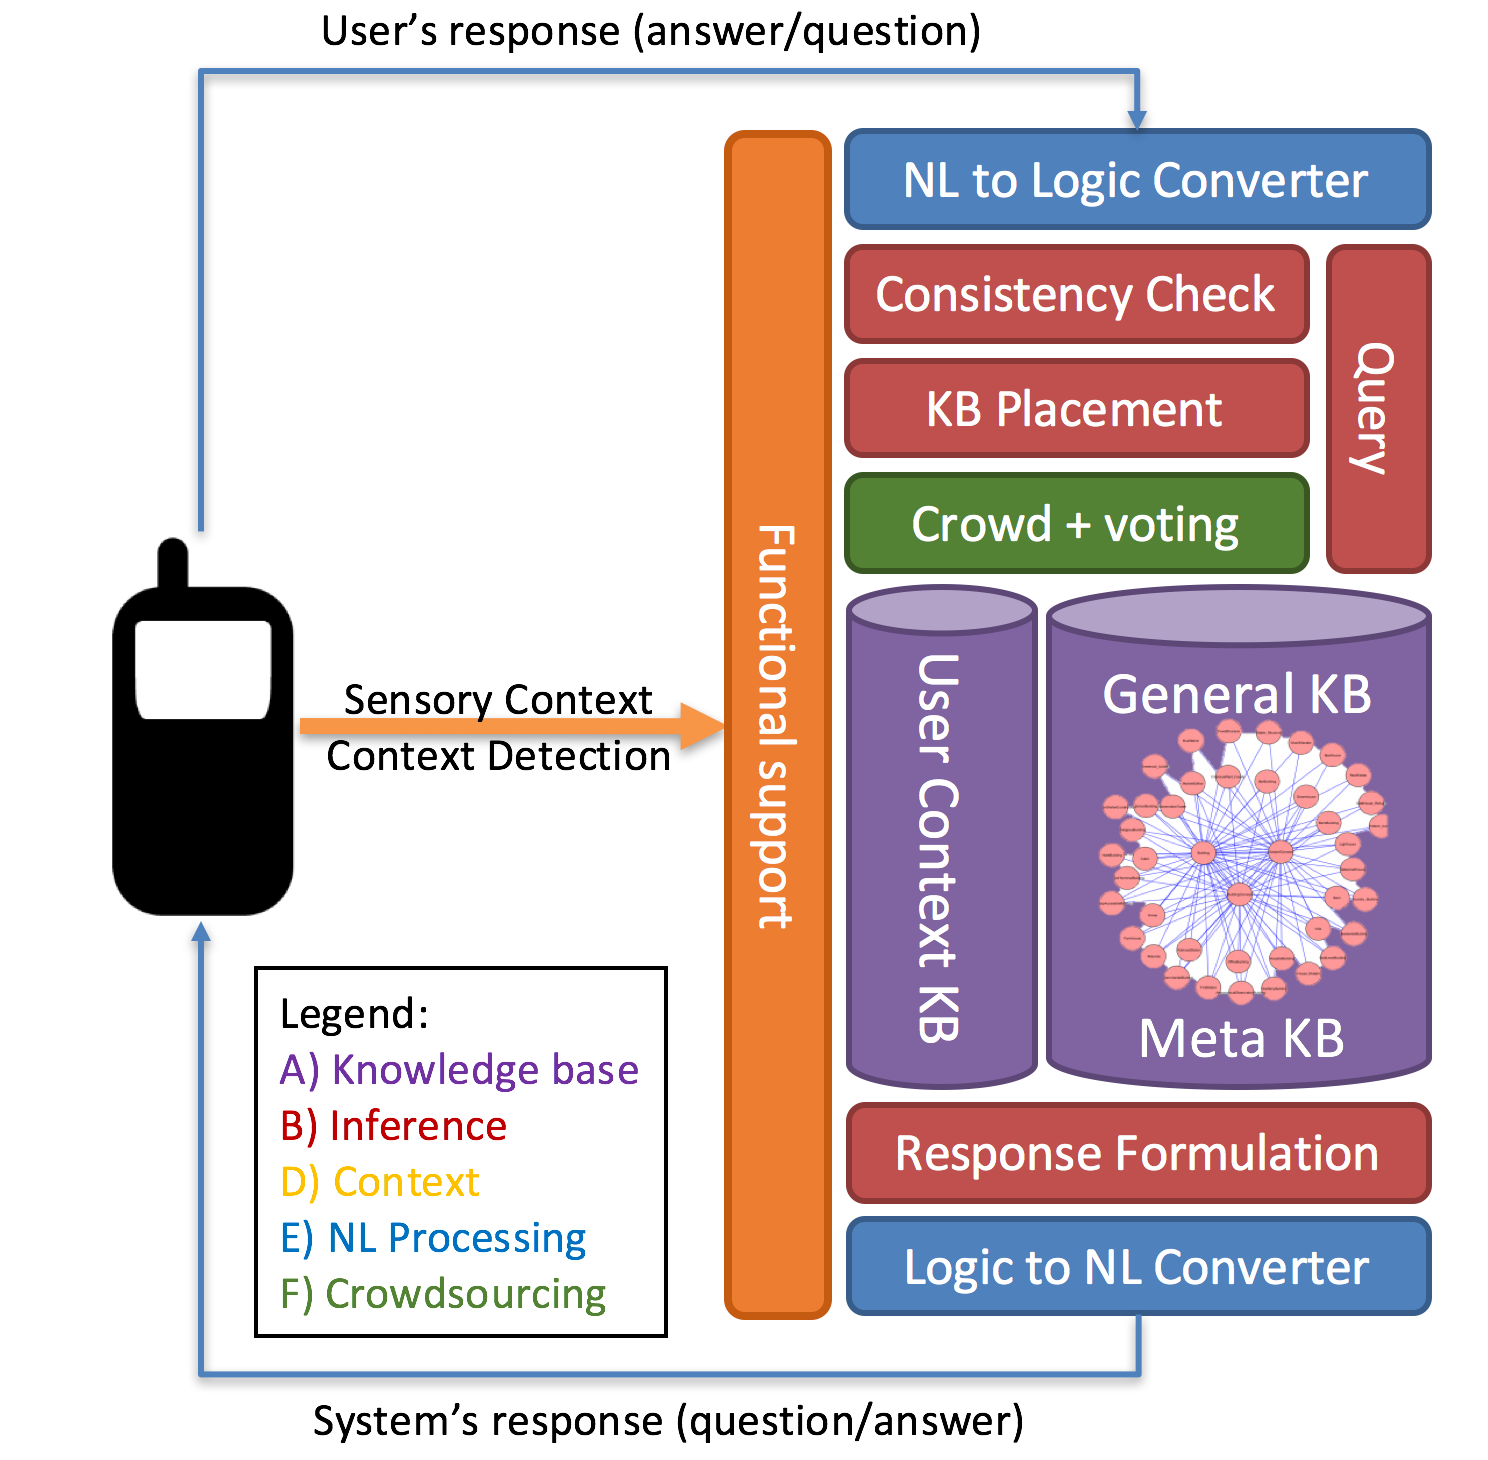
\includegraphics[width=1\textwidth]{figures/architecture.png}
	\caption{General Architecture of the KA system, with a simple interaction loop.}
	\label{fig:Architecture}
\end{figure}

Fig. 2. General Architecture of the KA system, with a simple interaction loop
At both ends of the stacked chain in Fig. 2, there are natural language processing components (marked in blue and with letter E), which are responsible for logic-to-language and language-to-logic conversion (sections 2.4 and 4.5). These are crucial if we want to interact with users in a natural way and thus avoid the need for users to be experts in first order logic. This module and its components are described in more detail in section 4.5.  
Besides the main interaction loop, which implicitly uses crowdsourcing while it interacts with the users, there is an additional component (marked in green and with letter F). This ?crowdsourcing and voting? component handles and decides, which elements of knowledge (logical assertions) can be safely asserted and made ?visible? to all the users and which are questionable and should stay visible only to the authors of the knowledge. If the piece of knowledge is questionable, the system marks it as such and then the question formulation process will check with other users whether it?s true or not. This is described in more detail in section 4.7.
In addition to logic-based components presented above, there is a functional driver system (marked in orange), which glues everything together, forwards the results of inference to the NL converters, accepts and asserts the context into the KB, handles the synchronization between the instances of the systems, etc.
%
% Fourth chapter 
%--------------------------------------------------------------------------------------------------
% 
\chapter{Real World Knowledge Acquisition Implementation}
%--------------------------------------------------------------------------------------------------

\section{Cyc}

TBW
%
% Fifth chapter 
%--------------------------------------------------------------------------------------------------
% 
\chapter{Evaluation}
%--------------------------------------------------------------------------------------------------
TBW

%
% If parts are used, the \chapteroutsidepart command must be called before final
 chapters that 
% regard all parts
%\chapteroutsidepart 
%
% Conclusions
%--------------------------------------------------------------------------------------------------
% 
\chapter{Conclusions}
%--------------------------------------------------------------------------------------------------

We came to the following conclusions \dots

%%%%%%%%%%%%%%%%%%%%%%%%%%%%%%%%%%%%%%%%%%%%%%%%%%%%%%%%%%%%%%%%%%%%%%%%%%%%%%%%
% Template Introduction

%%--------------------------------------------------------------------------------------------------
% 
\chapter{Introduction}
%--------------------------------------------------------------------------------------------------

\section{Thesis Structure}

The thesis should be structured as follows (note that while some parts are optional, their order is not):
\begin{itemize}
	\item \emph{Front Matter}
	\begin{itemize}
		\item Title pages
		\item Dedication (optional)
		\item Acknowledgments
		\item Abstract
		\item Povzetek
		\item Contents
		\item List of Figures (required if the thesis contains figures)
		\item List of Tables (required if the thesis contains tables)
		\item List of Algorithms (required if the thesis contains algorithms)
		\item Abbreviations (optional)
		\item Symbols (optional)
		\item Glossary (optional)
	\end{itemize}
	\item \emph{Main Matter}\footnote{The PhD thesis can also be divided into Parts --- this is not encouraged, but possible and supported by this template.}
	\begin{itemize}
		\item 1 Introduction
		\item $2, \dots, n-1$ Chapters
		\item $n$ Conclusions
	\end{itemize}
	The Introduction must clearly summarize the thesis from the topic application of the doctoral dissertation. The core text of the doctoral dissertation can be substituted by publications (or papers accepted for publication) in internationally recognized journals. In this case, the Introduction should clearly describe the scientific method and the candidate’s contribution to any publication which has been produced by several authors. In the Discussion or Conclusions, the candidate should summarize coherently the results of his/her dissertation.
	\item \emph{Appendices} (optional)
	\begin{itemize}
		\item Appendix A Title
		\item Appendix B Title
		\item \dots
	\end{itemize}
	If desired, the candidate can place some of his/her relevant papers in the appendices. In order to do so, he/she must obtain permissions from publishers.
	\item \emph{Back Matter}
	\begin{itemize}
		\item References
		\item Bibliography 
		\item Biography
		\item Index (optional)
	\end{itemize}
\end{itemize}

In addition, each author must prepare the cover page and spine using the two \texttt{.doc} files provided by IPS.

\section{Sectioning Example}

This is a section. Some more text. Some more text. Some more text. Some more text. Some more text. Some more text. Some more text. Some more text. Some more text. Some more text. Some more text. Some more text. 

Some more text. Some more text. Some more text. Some more text. Some more text. Some more text. Some more text. Some more text. Some more text. Some more text. Some more text. Some more text. 

\subsection{Subsection}

This is a subsection. Some more text. Some more text. Some more text. Some more text. Some more text. Some more text. Some more text. Some more text. Some more text. Some more text. Some more text. Some more text. 

Some more text. Some more text. Some more text. Some more text. Some more text. Some more text. Some more text. Some more text. Some more text. Some more text. Some more text. Some more text. 

\subsubsection{Subsubsection}

This is a subsubsection. Some more text. Some more text. Some more text. Some more text. Some more text. Some more text. Some more text. Some more text. Some more text. Some more text. Some more text. Some more text. 

Some more text. Some more text. Some more text. Some more text. Some more text. Some more text. Some more text. Some more text. Some more text. Some more text. Some more text. Some more text. 

\paragraph{Paragraph}

This is a paragraph. Some more text. Some more text. Some more text. Some more text. Some more text. Some more text. Some more text. Some more text. Some more text. Some more text. Some more text. Some more text.  

Some more text. Some more text. Some more text. Some more text. Some more text. Some more text. Some more text. Some more text. Some more text. Some more text. Some more text. Some more text. 

\subparagraph{Subparagraph}

This is a subparagraph. It is not possible to get deeper than this. Some more text. Some more text. Some more text. Some more text. Some more text. Some more text. Some more text. Some more text. Some more text. Some more text. Some more text. Some more text. 

Some more text. Some more text. Some more text. Some more text. Some more text. Some more text. Some more text. Some more text. Some more text. Some more text. Some more text. Some more text. 

\subparagraph{Subparagraph}

This is a subparagraph. It is not possible to get deeper than this. Some more text. Some more text. Some more text. Some more text. Some more text. Some more text. Some more text. Some more text. Some more text. Some more text. Some more text. Some more text. 

\paragraph{Paragraph}

This is a paragraph. Some more text. Some more text. Some more text. Some more text. Some more text. Some more text. Some more text. Some more text. Some more text. Some more text. Some more text. Some more text. 

\subsubsection{Subsubsection}

This is a subsubsection. Some more text. Some more text. Some more text. Some more text. Some more text. Some more text. Some more text. Some more text. Some more text. Some more text. Some more text. Some more text.  

\paragraph{Paragraph}

This is a paragraph. Some more text. Some more text. Some more text. Some more text. Some more text. Some more text. Some more text. Some more text. Some more text. Some more text. Some more text. Some more text.  

\paragraph{Paragraph}

This is a paragraph. Some more text. Some more text. Some more text. Some more text. Some more text. Some more text. Some more text. Some more text. Some more text. Some more text. Some more text. Some more text. 

\subsection{Subsection}

This is a subsection. Some more text. Some more text. Some more text. Some more text. Some more text. Some more text. Some more text. Some more text. Some more text. Some more text. Some more text. Some more text. 

\subsubsection{Subsubsection}

This is a subsubsection. Some more text. Some more text. Some more text. Some more text. Some more text. Some more text. Some more text. Some more text. Some more text. Some more text. Some more text. Some more text. 

\subsubsection{Subsubsection}

This is a subsubsection. Some more text. Some more text. Some more text. Some more text. Some more text. Some more text. Some more text. Some more text. Some more text. Some more text. Some more text. Some more text. 

%
% If needed, the thesis can consist of parts (not encouraged)
%\part{First Part of the Thesis}
%
% Second chapter 

%%--------------------------------------------------------------------------------------------------
% 
\chapter{Floating Bodies}
%--------------------------------------------------------------------------------------------------

Floating bodies are figures, tables and algorithms. 

\section{Figures}

Captions should be placed below figures as shown in \figurename~\ref{fig:ips-short}. If a caption is shorter than the line width, it should be centered. 

\begin{figure}[htb]
	\centering
		
\includegraphics[width=0.4\textwidth]{figures/ipslogo-cut.pdf}
	\caption{A large IPS logo.}
	\label{fig:ips-short}
\end{figure}

On the other hand, if a caption is very long (see \figurename~\ref{fig:ips-long}), only its first (short) part should be put in the List of Figures. 

\begin{figure}[htb]
	\centering
		
\includegraphics[width=0.15\textwidth]{figures/ipslogo-cut.pdf}
	\caption[A small IPS logo.]{A small IPS logo. The IPS has its own logo and a uniform graphic image, which is used on all its documents.}
	\label{fig:ips-long}
\end{figure}

\section{Tables}

Similar rules apply also to captions of tables, with the exception that captions are placed above tables (see \tablename~\ref{tab:example}).

\begin{table}[htb]
	\caption{A simple table.}
	\label{tab:example}
	\centering
		\begin{tabular}{ccc}
			\hline
			A & B & C \\
			\hline
			12 & 9834 & 327 \\
			51 & 2234 & 97 \\
			\hline
		\end{tabular}
\end{table}

\section{Algorithms}

Algorithm~\ref{alg:myalgorithm} presents an algorithm example. 

\begin{algorithm}[htb]
	\caption{An algorithm example.}
	\label{alg:myalgorithm}

	\vspace{5pt}
	\KwData{this text}
	\KwResult{complete understanding}
	\vspace{5pt}
	initialization\;
	\While{not at end of this document}{
		read current section\;
		\eIf{understood}{
			go to next section\;
			current section becomes this one\;
		}{
			go back to the beginning of current section\;
		}	
	}
\end{algorithm}

%
% Third chapter template

%%--------------------------------------------------------------------------------------------------
% 
\chapter{Equations and Measurement Units}
%--------------------------------------------------------------------------------------------------

\section{Equations}

Small equations are often written in-line (within the text), for example $j^\star = \sigma T^4$, while larger ones need to be displayed in the following way:
\begin{equation}
	\sigma = \frac{2 \pi^5 k^4}{15 c^2 h^3} = 5.6704 \times 10^{-8} J s^{-1} m^{-2} K^{-4}
	\label{eq:complex}
\end{equation}
All displayed equations need to be numbered so that they can be referenced later in the text (for example, Eq.~(\ref{eq:complex}) presents the Stefan's (or Stefan-Boltzmann) constant).

\section{Measurement Units}

The candidate can choose a standard for measurement units and has to consistently use it throughout the thesis. 

%
%\part{Second Part of the Thesis}
%
% Fourth chapter 

%%--------------------------------------------------------------------------------------------------
% 
\chapter{Definitions and Theorems}
%--------------------------------------------------------------------------------------------------

\section{Definitions}

See the formal definition of the right triangle in Definition~\ref{def:right-triangle}.

\begin{definition}[Right triangle]
\label{def:right-triangle}
A \emph{right triangle} is a triangle in which one angle is a 90-degree angle.
\end{definition}

\section{Theorems}
\label{sec:theorems}

The Pythagorean theorem is a relation in Euclidean geometry among the three sides of a right triangle. It states that the square of the hypotenuse (the side opposite the right angle) is equal to the sum of the squares of the other two sides \parencite{pythagoras}. \index{Pythagorean theorem!theorem}

\begin{theorem}[Pythagorean theorem]
\label{thm:pythagoras}
In every right triangle with sides $a$ and $b$ and hypotenuse $c$, the following holds:
\begin{equation}
a^2 + b^2 = c^2
\end{equation}
\end{theorem}

See Appendix~\ref{app:proofs} for the proof of this theorem.

%
% Fifth chapter 

%%--------------------------------------------------------------------------------------------------
% 
\chapter{Reference Formatting}
%--------------------------------------------------------------------------------------------------

References should be formatted using either the IEEE or APA 6th edition formatting style. This template uses the latter one. 

\section{IEEE}

Please see the template using the IEEE style. 

\section{APA 6th Edition}

References are cited using the \texttt{\textbackslash parencite} command. For example, see \parencite{mihailovic06}. The alternative \texttt{\textbackslash textcite} is used when the authors are mentioned in text. For example, let us cite the work by \textcite{depolli13}. References to journal articles that have not yet been published should contain the \texttt{doi}, as in \parencite{tusar14}.

Multiple references can be cited at the same time \parencite{kobal04,grace10,novak12eng,zupanc13}. Beside books and journal articles, parts of books \parencite{smodis09}, technical reports \parencite{ivekovic13eng}, PhD theses \parencite{dovgan14eng} and MSc theses \parencite{tusar07eng} can be included in the references.

Finally, on-line sources can be referenced, too, see Section~\ref{sec:theorems}.

%-------------------------------------------------------------------------------
%
% APPENDICES (optional)
%-------------------------------------------------------------------------------
%
%\appendix
%\begin{appendices}
%%
%% For example, proofs of theorems could be an appendix
%%-------------------------------------------------------------------------------
% 
\chapter{Proofs of Theorems}
\label{app:proofs}
%-------------------------------------------------------------------------------

\section{Proof of the Pythagorean Theorem}
\index{Pythagorean theorem!proof}

Let us prove the Pythagorean Theorem from page~\pageref{thm:pythagoras}.

\begin{proof}
This proof is based on the proportionality of the sides of two similar triangles, that is, upon the fact that the ratio of any two corresponding sides of similar triangles is the same regardless of the size of the triangles.

Let $ABC$ represent a right triangle, with the right angle located at $C$, as shown in Figure~\ref{fig:Pythagoras}. We draw the altitude from point $C$, and call $H$ its intersection with the hypotenuse $AB$. Point $H$ divides the length of the hypotenuse into two parts. 

\begin{figure}[htb]
	\centering
		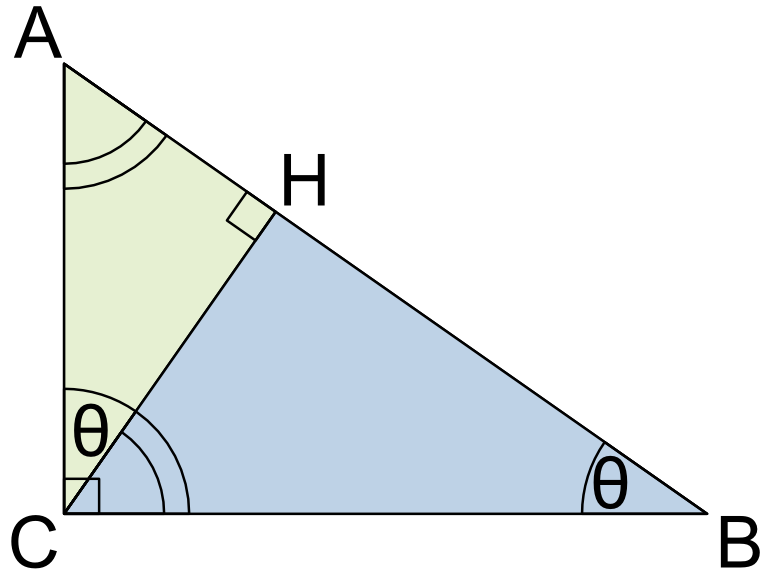
\includegraphics[width=0.3\textwidth]{figures/Pythagoras.png}
	\caption{Similar triangles used in the proof of the Pythagorean theorem.}
	\label{fig:Pythagoras}
\end{figure}

The new triangle $ACH$ is similar to triangle $ABC$, because they both have a right angle (by definition of the altitude), and they share the angle at $A$, meaning that the third angle will be the same in both triangles as well, marked as $\theta$ in Figure~\ref{fig:Pythagoras}. By a similar reasoning, the triangle $CBH$ is also similar to $ABC$. 

Similarity of the triangles leads to the equality of ratios of corresponding sides:
\begin{equation}
    \frac{BC}{AB}=\frac{BH}{BC} \text{ and } \frac{AC}{AB}=\frac{AH}{AC}.
\end{equation}
The first result equates $\cos \theta$ and the second result equates $\sin \theta$.

These ratios can be written as:
\begin{equation}
    {BC}^{2}={AB}\times {BH} \text{ and }{AC}^{2}={AB}\times {AH}.
\end{equation}
Summing these two equalities, we obtain:
\begin{equation}
    {BC}^{2}+{AC}^{2}={AB}\times {BH}+{AB}\times {AH}={AB}\times({AH}+{BH})={AB}^{2} ,
\end{equation}
which, tidying up, is the Pythagorean theorem:
\begin{equation}
    {BC}^{2}+{AC}^{2}={AB}^{2}.
\end{equation}
\end{proof}

%%
%\end{appendices}
%-------------------------------------------------------------------------------
%
% BACK MATTER
%-------------------------------------------------------------------------------
%
\backmatter
%
% References used in the thesis
\printreferences
% 
% Author's bibliography 
%-------------------------------------------------------------------------------
% 
\chapter{Bibliography}
%------------------------------------------------------------------------------
% Enclose with refsection and use \nocite{*}, if you need to list publications 
%not referenced in the thesis:
\begin{refsection}
\nocite{*}

\section*{Publications Related to the Thesis}

\defbibheading{subbibliography}{\subsection*{Journal Articles}}
\printbibliography[heading=subbibliography,keyword=myarticle]

\defbibheading{subbibliography}{\subsection*{Conference Paper}}
\printbibliography[heading=subbibliography,keyword=myconf]

\defbibheading{subbibliography}{\subsection*{Book Chapter}}
\printbibliography[heading=subbibliography,keyword=mybook]

\defbibheading{subbibliography}{\subsection*{Magazine Article}}
\printbibliography[heading=subbibliography,keyword=mymagazine]


%\section*{Other Publications (optional)}
%\dots

\end{refsection}

%
% Author's biography
%-------------------------------------------------------------------------------
% 
\chapter{Biography}
%-------------------------------------------------------------------------------

The author of this thesis is PhD candidate from Artificial Intelligence Lab at 
Jožef Stefan Institute, Slovenia. His research interests and PhD topic are in 
Natural Language Processing, Logical Inference, Knowledge Extraction and
Crowdsourcing. In 2010 he graduated from Faculty of Electrical Engineering and
started his doctoral studies at Jožef Stefan International Postgraduate School.
He worked as an Artificial Intelligence and Machine Learning researcher at
Jožef Stefan Artificial Intelligence Laboratory since 2005 on the topics related
to this thesis. From 2008 to 2013 he also worked as a principal software 
engineer for Cycorp Europe, which was at the time an EU branch of the American 
AI company Cyc Inc. During these years, he worked on an EU project developing 
distributed large scale inference engine (LarKC), and also on an AI assistant 
built on top of Cyc which lead to the development and implementation of the
approach described in this thesis. Some of the recent projects with a similar
topic include a concept of an intelligent motorhome (reasoning engine software 
interacting with sensors and actuators) for a European motorhome producer 
(Adria Mobil) and Named Entity Disambiguation algorithm which is a work in 
progress in collaboration with US Company Bloomberg L.P.

%
% Index (optional)
\printmyindex
%-------------------------------------------------------------------------------
\end{document}
